Array of time traces


New section? Fluctuations acting on background


% FIXME: Need reference
As seen from figure above, the fluctuations can be quite strong, something which has also been observed experimentally.
This is in fact something which should be taken into account when modelling the plasma.
% FIXME: Need reference
Models like Hasegawa-Wakatani are doing a split between background and fluctuations.
The free energy in the background gradients are driving the fluctuations, and only the fluctuations are kept track of.
As long as the background fluctuations are not severely altering the background gradients, this is a good approximation.
On the other hand, when the background gradients are altered, the drive for the fluctuations are also altered, and the fixed background approximation breaks down.
% FIXME: Need reference
Models like CYTO and CELMA does not do the separation of background and fluctuations, and one are with these models able to investigate how the fluctuations affect the background and not only the other way around.
We can do so by comparing the steady state profiles with the turbulent profiles.
A poloidal average and a temporal average containing the whole time series are done in order to get a good avergaged picture of the turbulent profile.
As apparent from figure
the background profiles are flattened
%
\begin{figure}[htb]
    \centering
    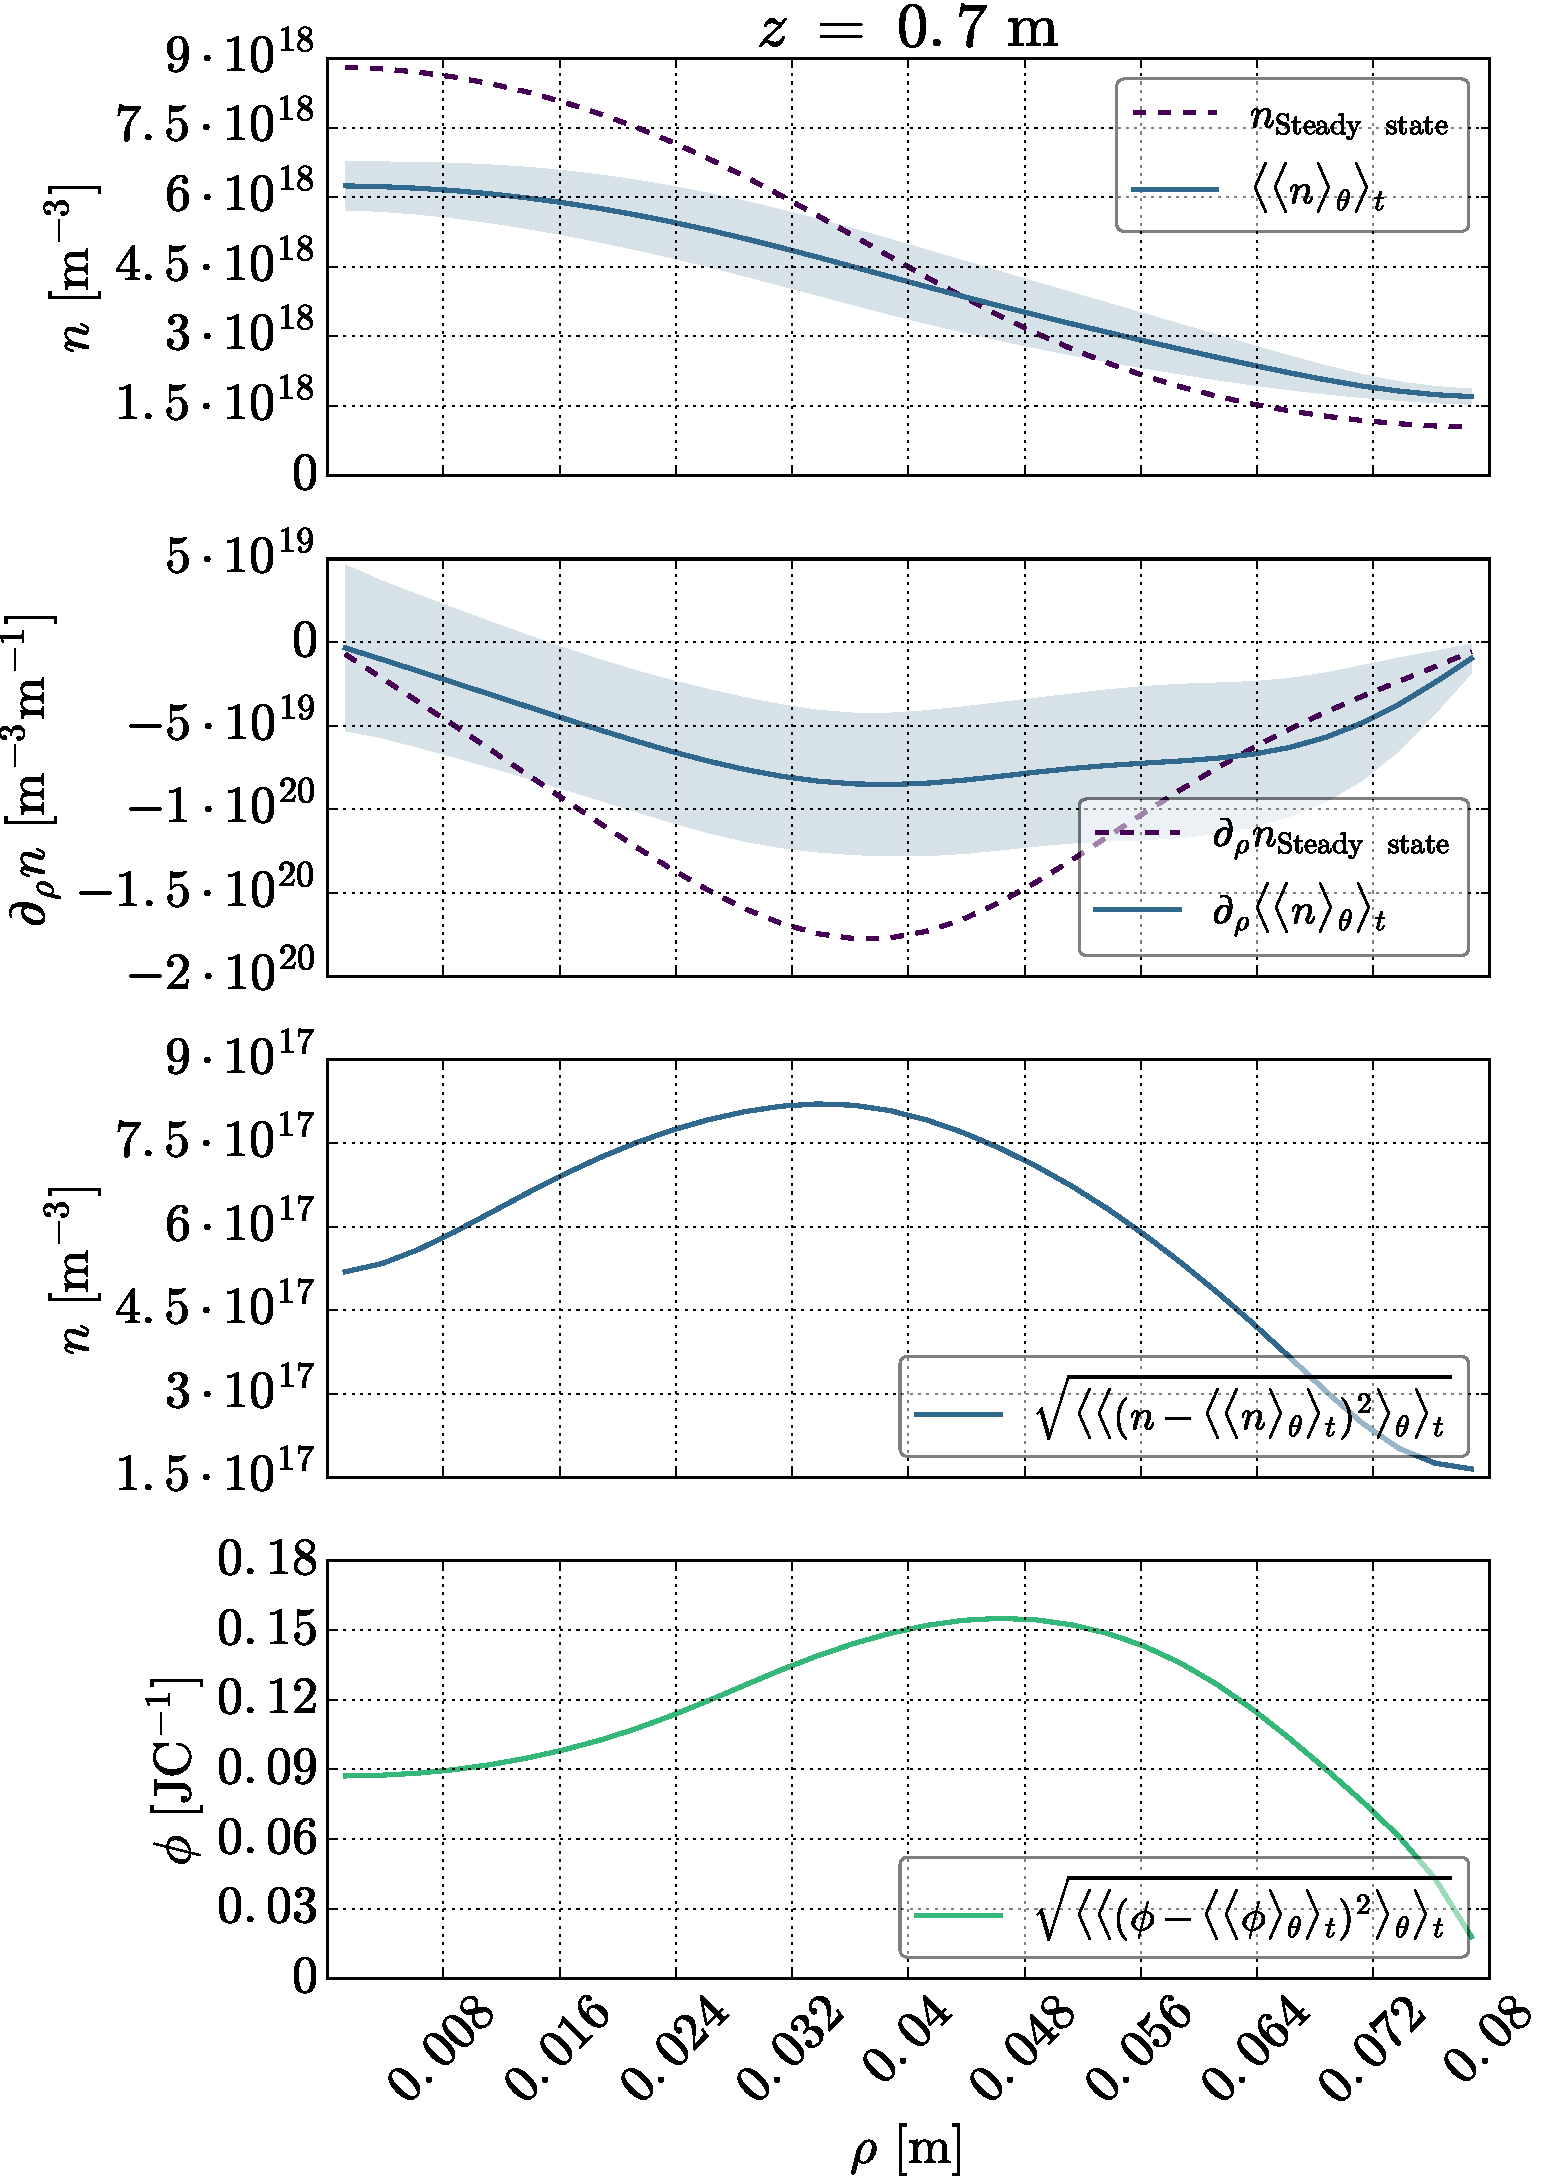
\includegraphics[width=1.0\textwidth]{fig/results/posOfFluct/posOfFluctB008}
    \caption{Flattening of the profiles together with the position of the fluctuations for $B=0.08\T$.
        The shaded area represents the standard deviation.
    }
    \label{fig:posOfFluct008}
\end{figure}
%
Need to discuss a bit more about
